\documentclass[12pt]{article}                         
\pagestyle{plain}

\usepackage{amsmath}     % Enhanced math environments (e.g., align).
\usepackage{amsfonts}    % Math fonts (e.g., \mathfrak{}).
\usepackage{amstext}     % Text inside math mode (e.g., \text{where}).
\usepackage{amssymb}     % Extra math symbols (e.g., \mathbb{R}).
\usepackage{array}       % Advanced table/array column definitions.
\usepackage{circledtext} % Puts text inside a circle (e.g., \circledtext{A}).
\usepackage{comment}     % Include/exclude blocks of text.
\usepackage{enumerate}   % Customize itemized/numbered lists.
\usepackage{geometry}    % Adjusts page margins and layout.
\usepackage{graphicx}    % Include images/graphics (\includegraphics).
\usepackage{latexsym}    % Access to basic LaTeX symbols.
\usepackage{multicol}    % Allows text columns on a page.
\usepackage{pgfplots}    % Create scientific plots from data (based on TikZ).
\usepackage{tabularx}    % Tables that stretch to page width.
\usepackage{tasks}       % Create multi-column lists.
\usepackage{textcomp}    % Provides many text symbols (e.g., \textcelsius).
\usepackage{tikz}        % Create vector graphics and diagrams.
\usepackage{xcolor}      % Define and use colors.
\usepackage{fancyhdr}
\geometry{a4paper, margin=1in}
\pagestyle{fancy}
\fancyhf{} % Clear all header and footer fields
\fancyhead[L]{Your Name} % Left header with name
\fancyhead[R]{October 07th 2025} % Right header with date
\renewcommand{\headrulewidth}{0.4pt} % Horizontal line below the header

\begin{document}

% Main title
\begin{center}
    \Large \textbf{Math 115E Activity 10} \\
    \vspace{0.2cm}
    \normalsize Chapter 4 Section 2 \\
    \normalsize Determining slope from two points
\end{center}

% ---STAR GRAPH----%
\begin{center}   
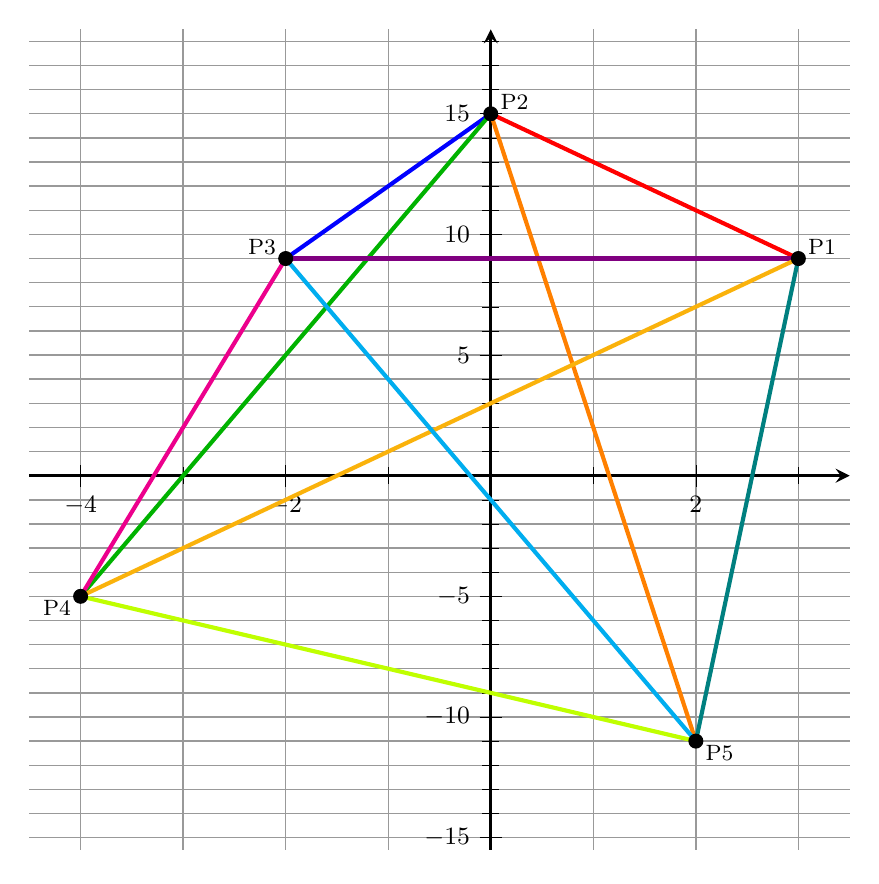
\begin{tikzpicture}
\begin{axis}[
    % Set the overall dimensions of the plot area
    height=12cm, 
    width=12cm,  
    % Set the domain and range for the axes
    xmin=-4.5, xmax=3.5,
    ymin=-15.5, ymax=18.5,
    % Manually set the tick marks
    xtick={-4,-2,0,2,4},
    ytick={-15,-10,-5,0,5,10,15,20},
    % Add 5 minor lines between each major tick on both axes
    minor x tick num=1,
    minor y tick num=4,
     % Axis and label styling
    axis lines=middle,
    tick label style={font=\small},
    % This command draws both major and minor grid lines
    grid=both,
    major grid style={line width=0.5pt,draw=gray!80},
    minor grid style={line width=0.5pt,draw=gray!80},
    % Axis and label styling
    axis lines=middle,
    tick style={draw=black, major tick length=8pt, minor tick length=6pt}, 
    xlabel style={at={(current axis.right of origin)}, anchor=west},
    ylabel style={at={(current axis.above origin)}, anchor=south},
    axis line style={-stealth, line width=1.2pt}
]

% --- LINES STARTING AT P1 (0, 15) ---
% 1. P1 to P2
\draw[line width=1.5pt, draw=red]      (axis cs:0,15) -- (axis cs:3,9);
% 2. P1 to P3
\draw[line width=1.5pt, draw=blue]     (axis cs:0,15) -- (axis cs:-2,9);
% 3. P1 to P4
\draw[line width=1.5pt, draw=green!70!black] (axis cs:0,15) -- (axis cs:-4,-5);
% 4. P1 to P5
\draw[line width=1.5pt, draw=orange]   (axis cs:0,15) -- (axis cs:2,-11);

% --- LINES STARTING AT P2 (3, 9) ---
% 5. P2 to P3
\draw[line width=1.5pt, draw=violet]   (axis cs:3,9) -- (axis cs:-2,9);
% 6. P2 to P4
\draw[line width=1.5pt, draw=yellow!70!red] (axis cs:3,9) -- (axis cs:-4,-5); % Gold/Ochre
% 7. P2 to P5
\draw[line width=1.5pt, draw=teal]     (axis cs:3,9) -- (axis cs:2,-11);

% --- LINES STARTING AT P3 (-2, 9) ---
% 8. P3 to P4
\draw[line width=1.5pt, draw=magenta]  (axis cs:-2,9) -- (axis cs:-4,-5);
% 9. P3 to P5
\draw[line width=1.5pt, draw=cyan]     (axis cs:-2,9) -- (axis cs:2,-11);

% --- LINE STARTING AT P4 (-4, -5) ---
% 10. P4 to P5
\draw[line width=1.5pt, draw=lime]     (axis cs:-4,-5) -- (axis cs:2,-11);

% --- 2. PLOT ALL 5 POINTS (Markers) ---
\addplot[only marks, mark=*, black, mark size=2.5pt] 
    coordinates {
        (0,15)
        (3,9)
        (2,-11)
        (-4,-5)
        (-2,9)
    };

% --- 3. ADD LABELS (P1, P2, P3, P4, P5) ---
\node[right, font=\footnotesize] at (axis cs:3,9.5) {P1};
\node[right, font=\footnotesize] at (axis cs:0,15.5) {P2};
\node[left, font=\footnotesize] at (axis cs:-2,9.5) {P3};
\node[left, font=\footnotesize] at (axis cs:-4,-5.5) {P4};
\node[right, font=\footnotesize] at (axis cs:2,-11.5) {P5};

\end{axis}
\end{tikzpicture}
\end{center}
% ----STAR GRAPH----%


% ---- SLOPE VALUE TO LETTER TABLE ---- %
\newcolumntype{W}{>{\centering\arraybackslash}p{0.7cm}} 
\setcounter{section}{1}
\section{Slope value to Letter table}
% --- Table 1: Columns 1-14 (14 columns) ---
\noindent % Prevents indentation before the table
\begin{tabularx}{\textwidth}{|*{14}{W|}} % 14 Left-aligned (L) columns
\hline
\textbf{-20} & \textbf{-15} & \textbf{-13} & \textbf{-11} & \textbf{-10} & \textbf{-9} & \textbf{-7} 
& \textbf{-6} & \textbf{-5} & \textbf{-4} & \textbf{-3} & \textbf{-2} & \textbf{-1} & \textbf{0} \\

J & Y & C & D & S & ? & Q & U & A & T
 & R & N & I & \_\_\_ \\
\hline
\end{tabularx}

\vspace{1em}

% --- Table 2: Columns 15-28 (14 columns) ---
\noindent
\begin{tabularx}{\textwidth}{|*{14}{W|}} % 14 Left-aligned (L) columns
\hline
\textbf{1} & \textbf{2} & \textbf{3} & \textbf{4} & \textbf{5} & \textbf{6} & \textbf{7} 
& \textbf{9} & \textbf{10} & \textbf{11} & \textbf{13} & \textbf{15} & \textbf{20} & \textbf{---} \\

G & H & V & K & E & L 
& B & Z & W & M & F & P & O & --- \\
\hline
\end{tabularx}
\renewcommand{\labelenumi}{\#\arabic{enumi}}
% ---- SLOPE VALUE TO LETTER TABLE ---- %


% ----  WRITE OUT THE SOLUTION ---- %
\newcolumntype{W}{>{\centering\arraybackslash}p{0.8cm}} 
\vspace{1cm}
\setcounter{section}{2}
\section{Write out the solution}
\noindent 
\rule{0.4cm}{0.4pt} \rule{0.4cm}{0.4pt} \rule{0.4cm}{0.4pt} 
\quad 
\rule{0.4cm}{0.4pt} 
\quad 
\rule{0.4cm}{0.4pt} \rule{0.4cm}{0.4pt} \rule{0.4cm}{0.4pt} \rule{0.4cm}{0.4pt} 
\quad
\rule{0.4cm}{0.4pt} \rule{0.4cm}{0.4pt} \rule{0.4cm}{0.4pt}
\quad 
\rule{0.4cm}{0.4pt} \rule{0.4cm}{0.4pt} \rule{0.4cm}{0.4pt} \rule{0.4cm}{0.4pt} \rule{0.4cm}{0.4pt} 
\quad 
\rule{0.4cm}{0.4pt} \rule{0.4cm}{0.4pt} \rule{0.4cm}{0.4pt} \rule{0.4cm}{0.4pt} \rule{0.4cm}{0.4pt} \rule{0.4cm}{0.4pt} 
\quad 
\rule{0.4cm}{0.4pt} :D
\\\\
\noindent
\begin{tabular}{|*{14}{W|}}  % 14 Left-aligned (L) columns
\hline
\textbf{\#7} & \textbf{\#9} & \textbf{\#1} & \textbf{\#2} & 
\textbf{\#10} & \textbf{\#2} & \textbf{\#3} & \textbf{\#9} & 
\textbf{\#5} & \textbf{\#6} & \textbf{\#2} & 
\textbf{\#12} & \textbf{\#15} & \textbf{\#4} \\

\hline
& & & & & & & & & & & & & \\
\hline
\end{tabular}

\vspace{1em}

% --- Table 2: Columns 15-28 (14 columns) ---
\noindent
\begin{tabular}{|*{14}{W|}}  % 14 Left-aligned (L) columns
\hline
\textbf{\#2} & \textbf{\#8} & \textbf{\#4} & \textbf{\#1} & \textbf{\#11} & 
\textbf{\#13} & \textbf{\#2} & \textbf{\#14} & \textbf{\#4} & 
\textbf{\#10} & \textbf{\#1} & \textbf{\#12} & 
\textbf{\#13} & \textbf{\#16} \\
\hline

& & & & & & & & & & & & & \\

\hline
\end{tabular}
% ----  WRITE OUT THE SOLUTION ---- %


% ---- COMMENTED OUT CYPHER ---- %
\begin{comment}
\section*{Line Table Key}
\noindent % Prevents indentation before the table
\begin{tabular}{|*{14}{W|}} 
\hline
% ROW 1: Empty Header Row
\textbf{\#7} & \textbf{\#9} & \textbf{\#1} & \textbf{\#2} & 
\textbf{\#10} & \textbf{\#2} & \textbf{\#3} & \textbf{\#9} & 
\textbf{\#5} & \textbf{\#6} & \textbf{\#2} & 
\textbf{\#12} & \textbf{\#15} & \textbf{\#20} \\

\hline
% ROW 2: Content Row - 14 items exactly
\textbf{C} & \textbf{A} & \textbf{N} & \textbf{\_} & 
\textbf{I} & \textbf{\_} & \textbf{H} & \textbf{A} & 
\textbf{V} & \textbf{E} & \textbf{\_} &
\textbf{T} & \textbf{W} & \textbf{O} \\
\hline
\end{tabular}

\vspace{1em} % Add vertical space between tables

% --- Table 2: Columns 15-28 (14 columns) ---
\noindent
\begin{tabular}{|*{14}{W|}} 
\hline
\textbf{\#8} & \textbf{\#4} & \textbf{\#1} & \textbf{\#11} & 
\textbf{\#13} & \textbf{\#2} & \textbf{\#14} & \textbf{\#4} & 
\textbf{\#10} & \textbf{\#1} & \textbf{\#12} & 
\textbf{\#13} & \textbf{\#16} & \textbf{:D} \\
\hline
% ROW 2: Letters - 13 Items exactly. The space is omitted for brevity.
\textbf{B} & \textbf{O} & \textbf{N} & \textbf{U} & 
\textbf{S} & \textbf{\_} & \textbf{P} & \textbf{O} & 
\textbf{I} & \textbf{N} & \textbf{T} & 
\textbf{S} & \textbf{?} & \textbf{:D} \\
\hline
\end{tabular}
\end{comment}
% ---- COMMENTED OUT CYPHER ---- %


% ---- FIND THE SLOPE OF EACH LINE STUDENT 1 ---- %
\vspace{10cm}
\setcounter{section}{0}
\section{Find the slope of each line}
\begin{minipage}[t]{0.6\textwidth}
    \begin{enumerate}
        \item (P1-P2) = %#1
        \\\\\\
        \item (P1-P3) = %#2
        \\\\\\
        \setcounter{enumi}{10} 
        \item = (\#10 - \#6) = %#11
        \\\\\\
    \end{enumerate}
\end{minipage}
\begin{minipage}[t]{0.6\textwidth}
    \begin{enumerate}[\#1]
        \setcounter{enumi}{8}
        \item (P3-P5) = %#9
        \\\\\\
        \item (P4-P5) = %#10
        \\\\\\
        \setcounter{enumi}{11} 
        \item = (\#1 - \#3) = %#12
        \\\\\\
    \end{enumerate}
\end{minipage}
\hrule
% ---- FIND THE SLOPE OF EACH LINE STUDENT 1 ---- %


% ---- FIND THE SLOPE OF EACH LINE STUDENT 2 ---- %

\setcounter{section}{0}
\section{Find the slope of each line}
\begin{minipage}[t]{0.6\textwidth}
    \begin{enumerate}
        \setcounter{enumi}{2} 
        \item (P1-P4) = %#3
        \\\\\\
        \item (P1-P5) = %#4
        \\\\\\
        \item = (P2-P3) = %#5
        \\\\\\
    \end{enumerate}
\end{minipage}
\begin{minipage}[t]{0.6\textwidth}
    \begin{enumerate}[\#1]
        \setcounter{enumi}{8}
        \setcounter{enumi}{12} 
        \item (\#7 + \#5) = %#13
        \\\\\\
        \item (\#9 + \#4) = %#14
        \\\\\\
        \\\\\\
    \end{enumerate}
\end{minipage}

\hrule 
% ---- FIND THE SLOPE OF EACH LINE STUDENT 2 ---- %


% ---- FIND THE SLOPE OF EACH LINE STUDENT 3 ---- %

\setcounter{section}{0}
\section{Find the slope of each line}
\begin{minipage}[t]{0.6\textwidth}
    \begin{enumerate}
        \setcounter{enumi}{5} 
        \item (P2-P4) = %#6
        \\\\\\
        \item (P2-P5) = %#7
        \\\\\\
        \item = (P3-P4) = %#8
        \\\\\\
    \end{enumerate}
\end{minipage}
\begin{minipage}[t]{0.6\textwidth}
    \begin{enumerate}[\#1]
        \setcounter{enumi}{14}
        \item $(\#3 \cdot \#6)$ = %#15
        \\\\\\
        \item $(\#1 - \#8)$ = %#16
        \\\\\\
        \\\\\\
    \end{enumerate}
\end{minipage}
% ---- FIND THE SLOPE OF EACH LINE STUDENT 3 ---- %



% ---- COMMENTED SOLUTIONS FOR SLOPE OF EACH LINE ---- %
\begin{comment}
\begin{minipage}[t]{0.6\textwidth}
    \begin{enumerate}
        \item (P1-P2) = \textbf{-2 == N}
        \\\\\\\\
        \item (P1-P3) = \textbf{0 == \_\_\_}
        \\\\\\\\
        \item (P1-P4) = \textbf{2 == H}
        \\\\\\\\
        \item (P1-P5) = \textbf{20 == O}
        \\\\\\\\
        \item (P2-P3) = \textbf{3 == V}
        \\\\\\\\
        \item (P2-P4) = \textbf{5 == E}
        \\\\\\\\
        \item (P2-P5) = \textbf{-13 == C}
        \\\\\\\\
        \item (P3-P4) = \textbf{7 == B}
    \end{enumerate}
\end{minipage}
\begin{minipage}[t]{0.6\textwidth}
    \begin{enumerate}[\#1]
        \setcounter{enumi}{8} % continues numbering
        \item (P3-P5) = \textbf{-5 == A}
        \\\\\\\\
        \item (P4-P5) = \textbf{-1 == I}
        \\\\\\\\
        \item = (\#10 - \#6) = \textbf{-6 == U}
        \\\\\\\\
        \item = (\#1 - \#3) = \textbf{-4 == T}
        \\\\\\\\
        \item = (\#7 + \#5) = \textbf{-10 == S}
        \\\\\\\\
        \item = (\#9 + \#4) =\textbf{15 == P}
        \\\\\\\\
        \item = (\#3 $\cdot$ \#6) = \textbf{10 == W }
        \\\\\\\\
        \item = (\#1 - \#8) = \textbf{-9 == ?}

    \end{enumerate}
\end{minipage}
\end{comment}
% ---- COMMENTED SOLUTIONS FOR SLOPE OF EACH LINE ---- %



\end{document}